

%%%%%%%%%%%%%%%%%%%%%%%%%%%%%%%%%%%%%%%%%

%----------------------------------------------------------------------------------------
%	PACKAGES AND THEMES
%----------------------------------------------------------------------------------------

\documentclass{beamer}

\mode<presentation> {

% The Beamer class comes with a number of default slide themes
% which change the colors and layouts of slides. Below this is a list
% of all the themes, uncomment each in turn to see what they look like.

%\usetheme{default}
%\usetheme{AnnArbor}
%\usetheme{Antibes}
%\usetheme{Bergen}
%\usetheme{Berkeley}
%\usetheme{Berlin}
%\usetheme{Boadilla}
%\usetheme{CambridgeUS}
%\usetheme{Copenhagen}
%\usetheme{Darmstadt}
%\usetheme{Dresden}
%\usetheme{Frankfurt}
%\usetheme{Goettingen}
%\usetheme{Hannover}
%\usetheme{Ilmenau}
%\usetheme{JuanLesPins}
%\usetheme{Luebeck}
\usetheme{Madrid}
%\usetheme{Malmoe}
%\usetheme{Marburg}
%\usetheme{Montpellier}
%\usetheme{PaloAlto}
%\usetheme{Pittsburgh}
%\usetheme{Rochester}
%\usetheme{Singapore}
%\usetheme{Szeged}
%\usetheme{Warsaw}

% As well as themes, the Beamer class has a number of color themes
% for any slide theme. Uncomment each of these in turn to see how it
% changes the colors of your current slide theme.

%\usecolortheme{albatross}
%\usecolortheme{beaver}
%\usecolortheme{beetle}
%\usecolortheme{crane}
%\usecolortheme{dolphin}
%\usecolortheme{dove}
%\usecolortheme{fly}
%\usecolortheme{lily}
%\usecolortheme{orchid}
%\usecolortheme{rose}
%\usecolortheme{seagull}
%\usecolortheme{seahorse}
%\usecolortheme{whale}
%\usecolortheme{wolverine}

%\setbeamertemplate{footline} % To remove the footer line in all slides uncomment this line
%\setbeamertemplate{footline}[page number] % To replace the footer line in all slides with a simple slide count uncomment this line

%\setbeamertemplate{navigation symbols}{} % To remove the navigation symbols from the bottom of all slides uncomment this line
}

\usepackage{graphicx} % Allows including images
\usepackage{booktabs} % Allows the use of \toprule, \midrule and \bottomrule in tables
\usepackage[vietnamese]{babel}
%----------------------------------------------------------------------------------------
%	TITLE PAGE
%----------------------------------------------------------------------------------------

\title[Presentation ]{Đồ án \#1 - VITON-HD
} % The short title appears at the bottom of every slide, the full title is only on the title page

\author{ Đinh Đức Anh Khoa - 23122001 \\ Nguyễn Lê Hoàng Trung - 23122002 \\ Nguyễn Đình Hà Dương - 23122004 \\ Đinh Đức Tài - 23122013
} % 

\institute[23TNT1] % Your institution as it will appear on the bottom of every slide, may be shorthand to save space
{
FIT@HCMUS \\ % Your institution for the title page
\medskip
\textit{TPHCM, tháng 12 năm 2023} % 
}
\date{} % Date, can be changed to a custom date

\begin{document}

\begin{frame}
\titlepage % Print the title page as the first slide
\end{frame}

\begin{frame}
\frametitle{Tổng quan} % Table of contents slide, comment this block out to remove it
\tableofcontents % Throughout your presentation, if you choose to use \section{} and \subsection{} commands, these will automatically be printed on this slide as an overview of your presentation
\end{frame}

%----------------------------------------------------------------------------------------
%	PRESENTATION SLIDES
%----------------------------------------------------------------------------------------
\section{Mở đầu} 
%________________Slide 1__________________
\begin{frame}
\frametitle{1. Mở đầu}
\begin{itemize}
\item Trong bài thuyết trình này, ta sẽ tìm hiểu về mô hình VITON-HD và các pre-trained model

\end{itemize}

\begin{figure}
    \centering
    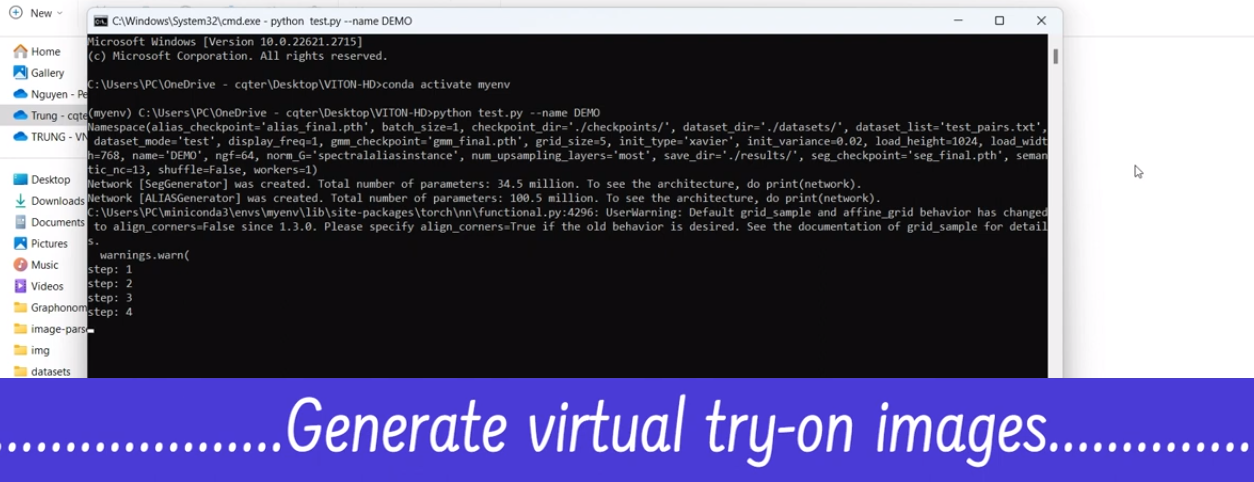
\includegraphics[width=1\linewidth]{images/opening.png}
    
    
\end{figure}

\end{frame}


\section{VITON-HD} 

\begin{frame}


\frametitle{2. VITON-HD}

\begin{figure}
    \centering
    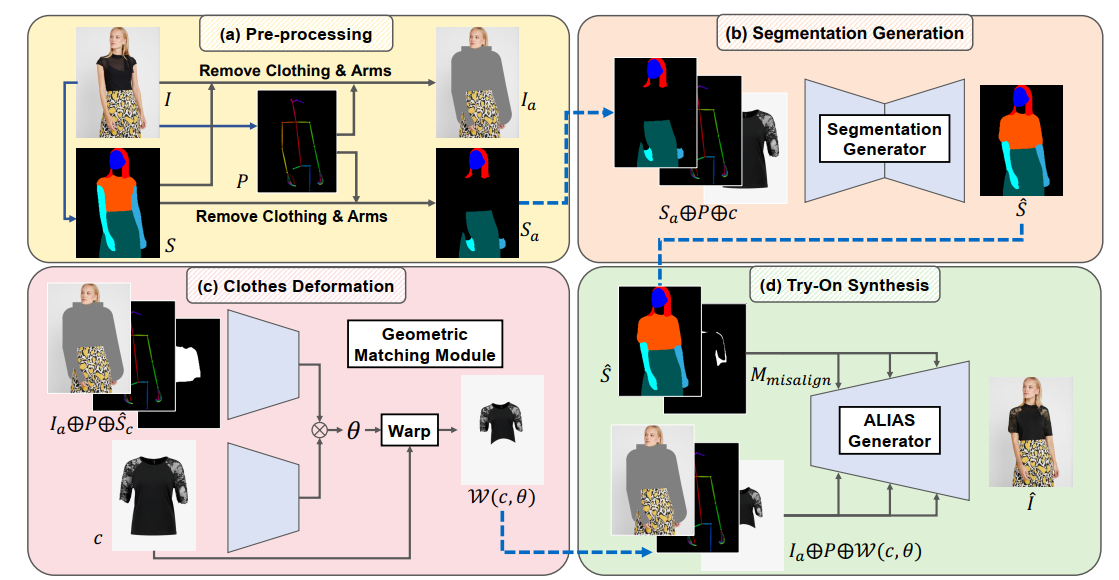
\includegraphics[width=1\linewidth]{images/vitonhd.png}
    
\end{figure}

\end{frame}

\begin{frame}
\frametitle{2. VITON-HD}
VITON-HD là một phương pháp mới trong lĩnh vực thử đồ ảo dựa trên hình ảnh. 
VITON-HD có khả năng chuyển đổi một món đồ cụ thể lên khu vực tương ứng trên cơ thể của một người với độ phân giải cao, đạt 1024×768 pixel.
\begin{itemize}
    \item Input: Ảnh người (\texttt{I}), bản đồ dáng người (\texttt{P} - định dạng \texttt{json} và \texttt{png}), bản đồ phân đoạn người (\texttt{S}), ảnh quần áo (\texttt{c}) và mask quần áo (\texttt{M\textsubscript{c}}).
    \item Output: Ảnh người mặc quần áo mới (\texttt{$\hat{I}$})
\end{itemize}
\end{frame}



\section{Segmentation Generator} 

\begin{frame}
\frametitle{3. Segmentation Generator}

\begin{figure}
    \centering
    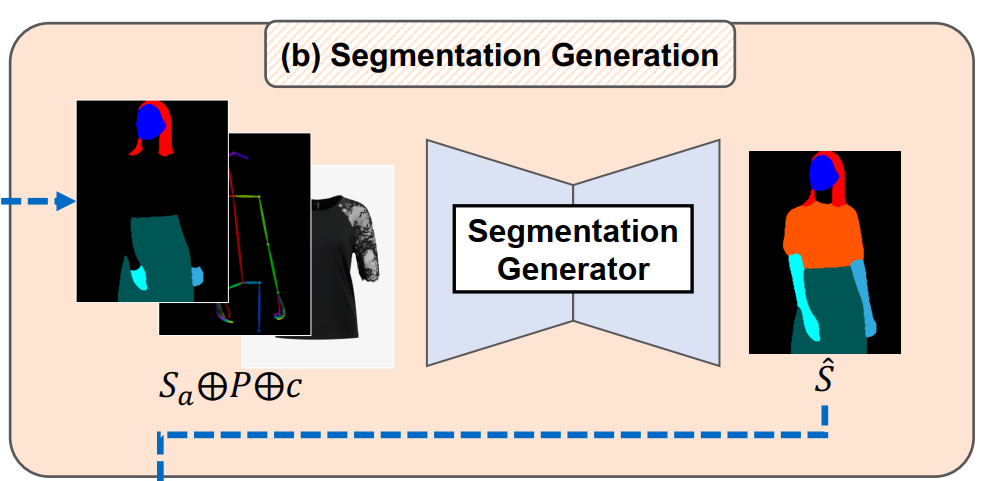
\includegraphics[width=1\linewidth]{seg.png}
    
    
\end{figure}

\end{frame}

\begin{frame}
\frametitle{3. Segmentation Generator}
\begin{itemize}
    \item Input: Bản đồ phân đoạn người (\texttt{S\textsubscript{a}}), bản đồ dáng người (\texttt{P}), ảnh quần áo cần thay (\texttt{c}) 
    \item Output: Bản đồ phân đoạn người mặc đồ \texttt{c} ($\hat{S}$)
\end{itemize}

\end{frame}

\section{Geometric Matching Module} 

\begin{frame}
\frametitle{4. Geometric Matching Module}

\begin{figure}
    \centering
    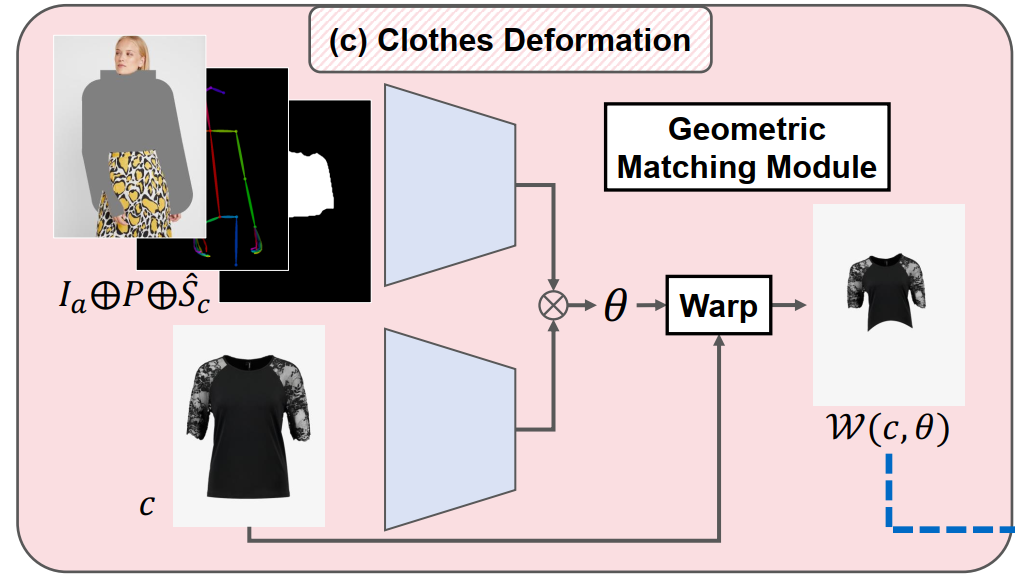
\includegraphics[width=1\linewidth]{gmm.png}
    
    
\end{figure}

\end{frame}

\begin{frame}
\frametitle{4. Geometric Matching Module}
\begin{itemize}
    \item Input: Hình ảnh người không phụ thuộc vào quần áo (\texttt{I\textsubscript{a}}), bản đồ dáng người (\texttt{P}), vùng quần áo của $\hat{S}$ (\texttt{$\hat{S}$\textsubscript{c}}), ảnh quần áo cần thay (\texttt{c}).
    \item Output: Ảnh quần áo được tinh chỉnh để vừa với cơ thể người (\texttt{W(c,$\theta$)})
\end{itemize}
\end{frame}

\section{ALIgnment-Aware Segment (ALIAS) Generator} 

\begin{frame}
\frametitle{5. ALIAS Generator}

\begin{figure}
    \centering
    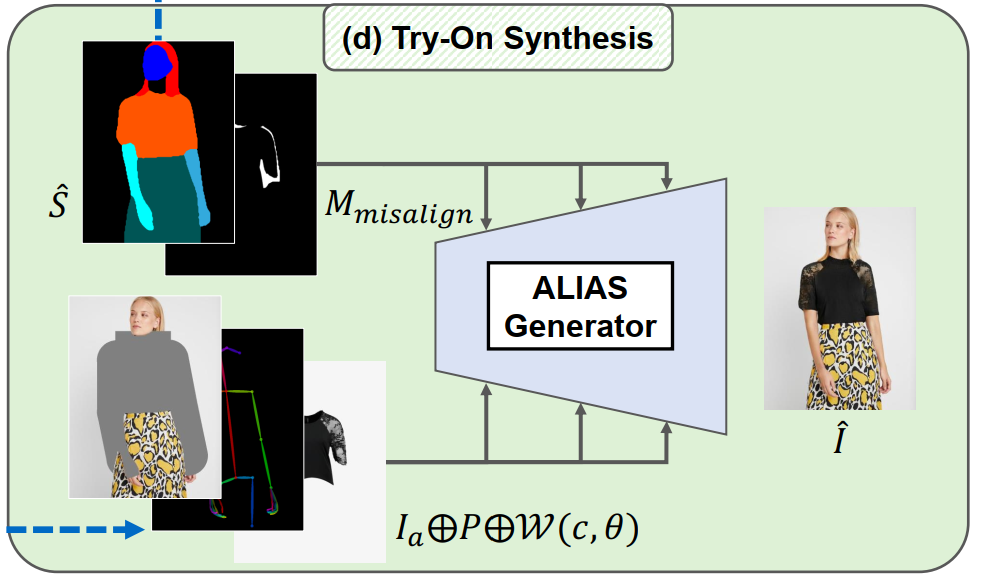
\includegraphics[width=1\linewidth]{alias.png}
    
    
\end{figure}

\end{frame}

\begin{frame}
\frametitle{5. ALIAS Generator}
\begin{itemize}
    \item Input: Bản đồ phân đoạn người mặc đồ \texttt{c} ($\hat{S}$), mask sai lệch nhị phân (\texttt{M\textsubscript{misalign}}), hình ảnh người không phụ thuộc vào quần áo (\texttt{I\textsubscript{a}}), bản đồ dáng người (\texttt{P}), ảnh quần áo được tinh chỉnh vừa với cơ thể người (\texttt{W(c,$\theta$)}).
    \\Mask sai lệch nhị phân - misalignment binary mask (\texttt{M\textsubscript{misalign}}) được tạo bằng cách loại trừ mask của ảnh quần áo \texttt{c} đã được tinh chỉnh (\texttt{W(M\textsubscript{c},$\theta$)}) khỏi vùng quần áo của $\hat{S}$ (\texttt{$\hat{S}$\textsubscript{c}}) theo công thức sau:
    \begin{enumerate}
        \item \texttt{M\textsubscript{align}} = $\hat{S}$\textsubscript{c} $\cap$ \texttt{W(M\textsubscript{c},$\theta$)}, trong đó M\textsubscript{c} là mask của quần áo \texttt{c} cần thay
        \item \texttt{M\textsubscript{misalign}} = $\hat{S}$\textsubscript{c} - \texttt{M\textsubscript{align}}
    \end{enumerate}
    \par
    \item Output: Ảnh người mặc đồ mới ($\hat{I}$)
\end{itemize}
\end{frame}

\begin{frame}
\frametitle{5.1 ALIAS normalization}

\begin{figure}
    \centering
    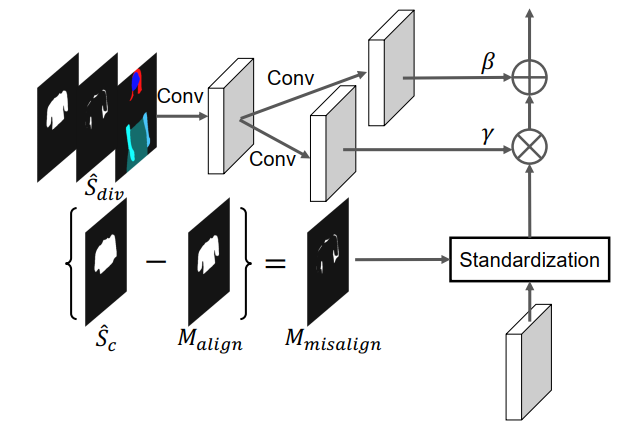
\includegraphics[width=1\linewidth]{alias_n.png}
    
    
\end{figure}

\end{frame}

\begin{frame}
\frametitle{5.2 ALIAS generator}

\begin{figure}
    \centering
    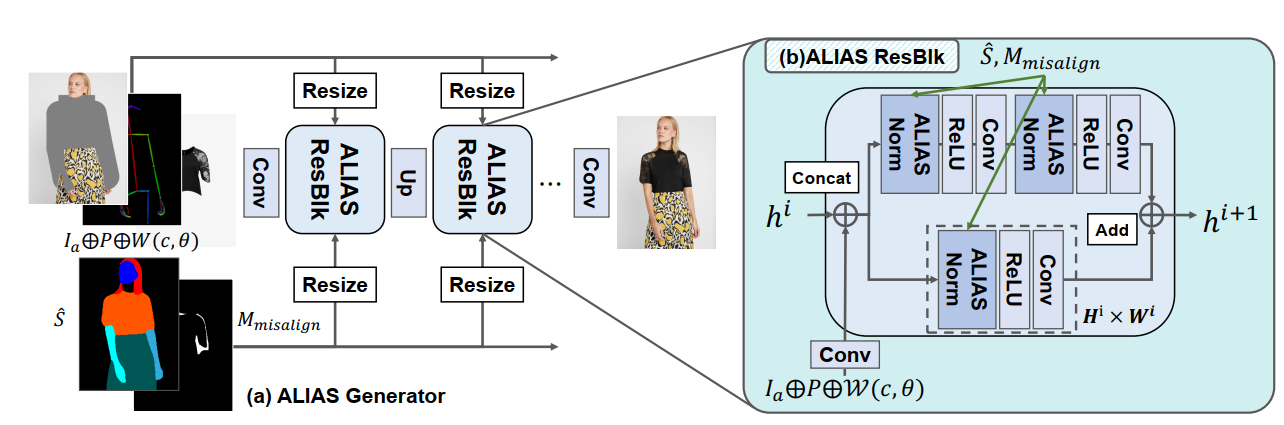
\includegraphics[width=1\linewidth]{alias_ge.png}
    
    
\end{figure}

\end{frame}


%------------------------------------------------
%_________________Slide 6. ______________________
\begin{frame}
\frametitle{Tham Khảo}

\begin{itemize}
    \item VITON-HD: High-Resolution Virtual Try-On via Misalignment-Aware Normalization
\end{itemize}


\end{frame}

\begin{frame}
\Huge{\centerline{The End}}
\end{frame}

%----------------------------------------------------------------------------------------

\end{document} 